%iffalse
\let\negmedspace\undefined
\let\negthickspace\undefined
\documentclass[journal,12pt,onecolumn]{IEEEtran}
\usepackage{cite}
\usepackage{amsmath,amssymb,amsfonts,amsthm}
\usepackage{algorithmic}
\usepackage{graphicx}
\usepackage{textcomp}
\usepackage{xcolor}
\usepackage{txfonts}
\usepackage{listings}
\usepackage{enumitem}
\usepackage{enumitem,multicol}
\usepackage{mathtools}
\usepackage{gensymb}
\usepackage{comment}
\usepackage[breaklinks=true]{hyperref}
\usepackage{tkz-euclide} 
\usepackage{listings}
\usepackage{gvv}                                        
%\def\inputGnumericTable{}                                 
\usepackage[latin1]{inputenc}                                
\usepackage{color}                                            
\usepackage{array}                                            
\usepackage{longtable}                                       
\usepackage{calc}                                             
\usepackage{multirow}                                         
\usepackage{hhline}                                           
\usepackage{ifthen}                                           
\usepackage{lscape}
\usepackage{tabularx}
\usepackage{array}
\usepackage{float}
\usepackage[american,siunitx]{circuitikz}
\usetikzlibrary{arrows,shapes,calc,positioning}
\usepackage{pgfplots}


\newtheorem{theorem}{Theorem}[section]
\newtheorem{problem}{Problem}
\newtheorem{proposition}{Proposition}[section]
\newtheorem{lemma}{Lemma}[section]
\newtheorem{corollary}[theorem]{Corollary}
\newtheorem{example}{Example}[section]
\newtheorem{definition}[problem]{Definition}
\newcommand{\BEQA}{\begin{eqnarray}}
\newcommand{\EEQA}{\end{eqnarray}}
\newcommand{\define}{\stackrel{\triangle}{=}}
\theoremstyle{remark}
\newtheorem{rem}{Remark}
\pgfplotsset{compat=1.18}

% Marks the beginning of the document
\begin{document}
\bibliographystyle{IEEEtran}
\vspace{3cm}

\title{XE-2022}
\author{EE24Btech11022 - Eshan Sharma}
\maketitle

\renewcommand{\thefigure}{\theenumi}
\renewcommand{\thetable}{\theenumi}



\begin{enumerate}
\item A two-dimensional potential flow solution for flow past an airfoil has a streamline pattern as shown in the figure. Which of the following conditions is additionally required to satisfy the Kutta condition?

\begin{center}
	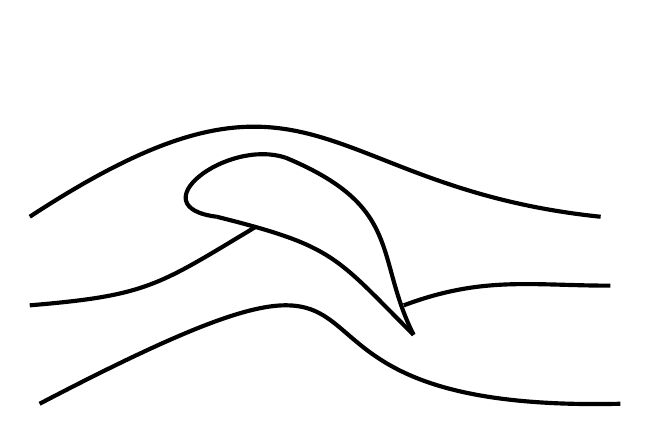
\begin{tikzpicture}[scale = 0.5]
		\tikzstyle{every node}=[font=\LARGE]
		\draw [line width=1.5pt, short] (5.5,13.75) .. controls (12.75,18.5) and (12.75,14.5) .. (20,13.75);
		\draw [line width=1.5pt, short] (5.75,9) .. controls (16.75,14.75) and (9.75,8.75) .. (20.5,9);
		\draw [line width=1.5pt, short] (5.5,11.5) .. controls (8.5,11.75) and (8.75,12) .. (11.25,13.5);
		\draw [line width=1.5pt, short] (15,11.5) .. controls (17,12.25) and (18.25,12) .. (20.25,12);
		\draw [line width=1.5pt, short] (10.25,13.75) .. controls (13.25,13) and (13.25,12.75) .. (15.25,10.75);
		\draw [line width=1.5pt, short] (15.25,10.75) .. controls (14.25,12.75) and (15,14) .. (12,15.25);
		\draw [line width=1.5pt, short] (12,15.25) .. controls (10.5,15.75) and (8.25,14) .. (10.25,13.75);
	\end{tikzpicture}
\end{center}

\begin{enumerate}
	\item Addition of a source of strength $Q > 0$
	\item Addition of a source of strength $Q < 0$
	\item Addition of a circulation of strength $\Gamma > 0$ (counter-clockwise)
	\item Addition of a circulation of strength $\Gamma < 0$ (clockwise)
\end{enumerate}

\item Consider the Blasius solution for the incompressible laminar flat plate boundary layer. Among the following options, select the correct relation for the development of the momentum thickness $\Theta$ with distance $X$ from the leading edge along the length of the plate.

\begin{enumerate}
	\item $\Theta \propto X^{2/3}$
	\item $\Theta \propto X^{1/2}$
	\item $\Theta \propto X^{1/7}$
	\item $\Theta \propto X^{-2/3}$
\end{enumerate}

\item In a two-dimensional potential flow, the doublet is a limit of the superposition of

\begin{enumerate}
	\item a uniform stream and a source
	\item a source and a sink of equal strength
	\item a uniform stream and a sink
	\item a source and a vortex
\end{enumerate}

 \item An ideal glider has drag characteristics given by $C_D = C_{D_0} + C_{D_i}$, where
$C_{D_i} = K C_L^2$ is the induced drag coefficient, $C_L$ is the lift coefficient, and $K$ is a constant. For maximum range of the glider, the ratio $C_{D_0} / C_{D_i}$ is
\begin{enumerate}
	\item 1
	\item $\frac{1}{3}$
	\item 3
	\item $\frac{3}{2}$
\end{enumerate}

\item The figures shown in the options are schematics of airfoil shapes (not to scale). For a civilian transport aircraft designed for a cruise Mach number of 0.8, which among them is aerodynamically best suited as a wing section?
\begin{enumerate}
	\item \begin{minipage}{0.25\textwidth}
		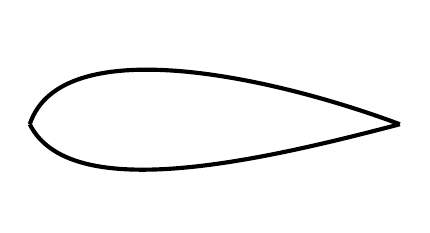
\begin{tikzpicture}[scale = 0.4]
			\tikzstyle{every node}=[font=\LARGE]
			\draw [line width=1.5pt, short] (6.75,13) .. controls (7.75,16) and (14.5,14.5) .. (18.5,13);
			\draw [line width=1.5pt, short] (6.75,13) .. controls (8,10.5) and (13.75,11.75) .. (18.5,13);
		\end{tikzpicture}
	\end{minipage}
	
	\item \begin{minipage}{0.25\textwidth}
		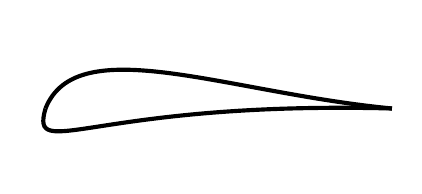
\begin{tikzpicture}[scale = 0.4]
			\tikzstyle{every node}=[font=\LARGE]
			\draw [line width=1.5pt, short] (6,13.5) .. controls (7,16) and (11.75,14) .. (17,13.5);
			\draw [line width=1.5pt, short] (6,13.5) .. controls (5.5,11.75) and (7.5,13.75) .. (17,13.5);
		\end{tikzpicture}
	\end{minipage}
	
	\item \begin{minipage}{0.25\textwidth}
		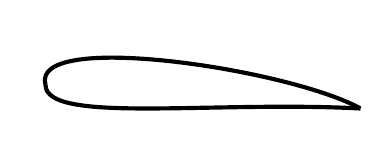
\begin{tikzpicture}[scale = 0.4]
			\tikzstyle{every node}=[font=\Large]
			\draw [line width=1.5pt, short] (7.5,13) .. controls (7,14.75) and (15.25,13.5) .. (17.5,12.25);
			\draw [line width=1.5pt, short] (17.5,12.25) .. controls (12.75,12.5) and (7.5,11.75) .. (7.5,13);
		\end{tikzpicture}
	\end{minipage}
	
	\item \begin{minipage}{0.25\textwidth}
		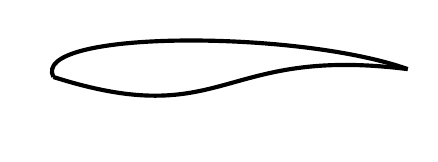
\begin{tikzpicture}[scale = 0.4]
			\tikzstyle{every node}=[font=\LARGE]
			\draw [line width=1.5pt, short] (7,13.25) .. controls (6.25,14.75) and (14.75,14.75) .. (18.25,13.5);
			\draw [line width=1.5pt, short] (7,13.25) .. controls (12.5,11.5) and (12.25,14.25) .. (18.25,13.5);
		\end{tikzpicture}
	\end{minipage}

\end{enumerate}

\item For a longitudinally statically stable aircraft, which one of the following represents the relationship between the coefficient of pitching moment about the center of gravity $C_{m_{cg}}$ and absolute angle of attack $\alpha_a$?

(Note: nose-up moment is positive.)

\begin{enumerate}
	\item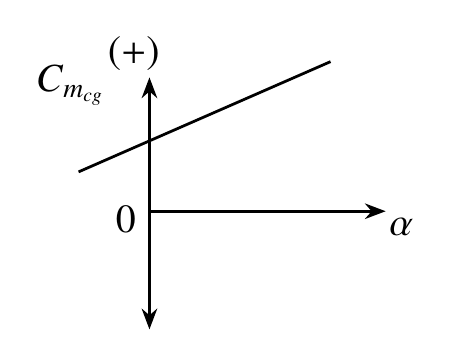
\begin{tikzpicture}[scale = 0.4]
			\tikzstyle{every node}=[font=\Large]
			\draw [line width=1pt, <->, >=Stealth] (8,16.5) -- (8,8.5);
			\draw [line width=1pt, ->, >=Stealth] (8,12.25) -- (15.5,12.25);
			\draw [line width=1pt, short] (5.75,13.5) -- (13.75,17);
			\node [font=\Large] at (7.25,12) {0};
			\node [font=\Large] at (7.5,17.25) {(+)};
			\node [font=\Large] at (16,11.75) {$\alpha$};
			\node [font=\Large] at (5.5,16.25) {$C_{m_{cg}}$};
		\end{tikzpicture}
	\item 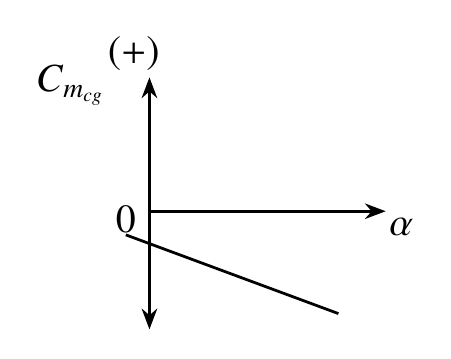
\begin{tikzpicture}[scale = 0.4]
		\tikzstyle{every node}=[font=\Large]
		\draw [line width=1pt, <->, >=Stealth] (8,16.5) -- (8,8.5);
		\draw [line width=1pt, ->, >=Stealth] (8,12.25) -- (15.5,12.25);
		\node [font=\Large] at (7.25,12) {0};
		\node [font=\Large] at (7.5,17.25) {(+)};
		\node [font=\Large] at (16,11.75) {$\alpha$};
		\node [font=\Large] at (5.5,16.25) {$C_{m_{cg}}$};
		\draw [line width=1pt, short] (7.25,11.5) -- (14,9);
		\end{tikzpicture}
	\item 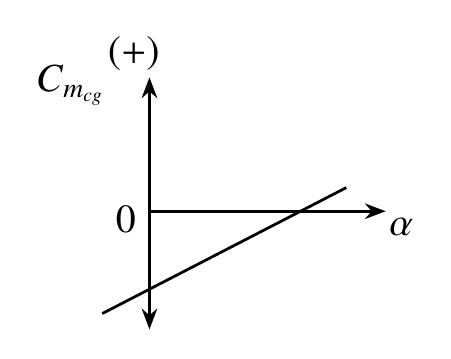
\begin{tikzpicture}[scale = 0.4]
		\tikzstyle{every node}=[font=\Large]
		\draw [line width=1pt, <->, >=Stealth] (8,16.5) -- (8,8.5);
		\draw [line width=1pt, ->, >=Stealth] (8,12.25) -- (15.5,12.25);
		\node [font=\Large] at (7.25,12) {0};
		\node [font=\Large] at (7.5,17.25) {(+)};
		\node [font=\Large] at (16,11.75) {$\alpha$};
		\node [font=\Large] at (5.5,16.25) {$C_{m_{cg}}$};
		\draw [line width=1pt, short] (6.5,9) -- (14.25,13);
		\end{tikzpicture}
	\item 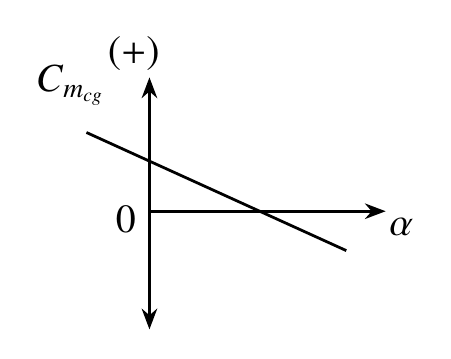
\begin{tikzpicture}[scale = 0.4]
		\tikzstyle{every node}=[font=\Large]
		\draw [line width=1pt, <->, >=Stealth] (8,16.5) -- (8,8.5);
		\draw [line width=1pt, ->, >=Stealth] (8,12.25) -- (15.5,12.25);
		\node [font=\Large] at (7.25,12) {0};
		\node [font=\Large] at (7.5,17.25) {(+)};
		\node [font=\Large] at (16,11.75) {$\alpha$};
		\node [font=\Large] at (5.5,16.25) {$C_{m_{cg}}$};
		\draw [line width=1pt, short] (6,14.75) -- (14.25,11);
		\end{tikzpicture}
\end{enumerate}

\item In a single-spool aviation turbojet engine, which of the following is the correct relationship between the total work output $W_t$ of a 2-stage axial turbine and the total work required $W_c$ by a 6-stage axial compressor, neglecting losses?

\begin{enumerate}
	\item $W_t = 2 W_c$
	\item $W_t = 6 W_c$
	\item $W_t = W_c$
	\item $W_t = 3 W_c$
\end{enumerate}

\item For a stage of a 50\% reaction ideal axial flow compressor (symmetrical blading), select the correct statement from the options given.

\begin{enumerate}
	\item The stagnation enthalpy rise across the rotor is 50\% of the rise across the stage.
	\item The static enthalpy rise across the rotor is 50\% of the rise across the stage.
	\item Axial velocity component of the flow at the rotor exit is 50\% of that at the rotor entry.
	\item The static pressure rise across the rotor is 50\% of the rise across the stator.
\end{enumerate}

\item An aircraft is cruising with a forward speed $V_a$ and the jet exhaust speed relative to the engine at the exit is $V_j$. If $\frac{V_j}{V_a} = 2$, what is the propulsive efficiency?

\begin{enumerate}
	\item 0.50
	\item 1.00
	\item 0.33
	\item 0.67
\end{enumerate}

\item Consider the four basic symmetrical flight loading conditions corresponding to the corners of a typical V-n diagram. For one of these flight loading conditions, it is observed that (i) the compressive bending stresses have a maximum value in the bottom aft region (see figure) of the wing cross-section; and (ii) the tensile bending stresses are maximum in the upper forward region (see figure) of the wing cross-section. For the preceding observations, select the corresponding flight loading condition from the options given.

\begin{center}
	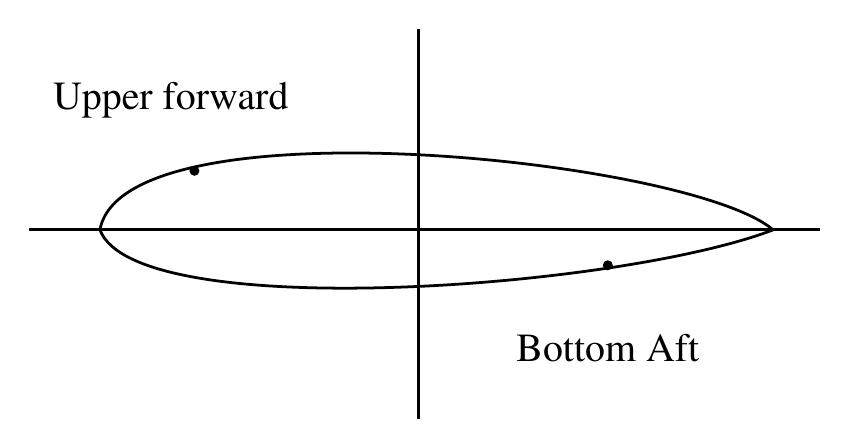
\begin{tikzpicture}[scale = 0.6]
	\tikzstyle{every node}=[font=\Large]
	\draw [line width=1pt, short] (10,16.75) -- (10,8.5);
	\draw [line width=1pt, short] (1.75,12.5) -- (18.5,12.5);
	\draw [line width=1pt, short] (3.25,12.5) .. controls (3.75,15.25) and (15.75,14) .. (17.5,12.5);
	\draw [line width=1pt, short] (3.25,12.5) .. controls (4,10.5) and (14.25,11.25) .. (17.5,12.5);
	\node at (5.25,13.75) [circ] {};
	\node at (14,11.75) [circ] {};
	\node [font=\Large] at (4.75,15.25) {Upper forward};
	\node [font=\Large] at (14,10) {Bottom Aft};	
	\end{tikzpicture}
\end{center}

\begin{enumerate}
	\item Positive high angle of attack
	\item Positive low angle of attack
	\item Negative high angle of attack
	\item Negative low angle of attack
\end{enumerate}

\item Which one of the following figures represents the qualitative variation of absolute deceleration $|\frac{dV}{dt}|$ with altitude $h$ (measured from the mean sea level) for a space vehicle undergoing a ballistic entry into the Earth?s atmosphere?

\begin{enumerate}
	\item 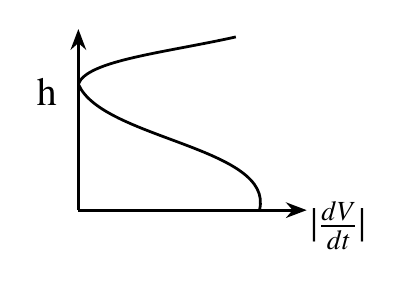
\begin{tikzpicture}[scale = 0.4]
		\tikzstyle{every node}=[font=\Large]
		\draw [line width=1pt, ->, >=Stealth] (7.5,11.5) -- (7.5,17.25);
		\draw [line width=1pt, ->, >=Stealth] (7.5,11.5) -- (14.75,11.5);
		\node [font=\Large] at (6.5,15.25) {h};
		\node [font=\Large] at (15.75,11) {$|\frac{dV}{dt}|$};
		\draw [line width=1pt, short] (12.5,17) .. controls (10.25,16.5) and (7.75,16.25) .. (7.5,15.5);
		\draw [line width=1pt, short] (7.5,15.5) .. controls (8.25,13.75) and (13.75,13.5) .. (13.25,11.5);
		\end{tikzpicture}

	
	\item 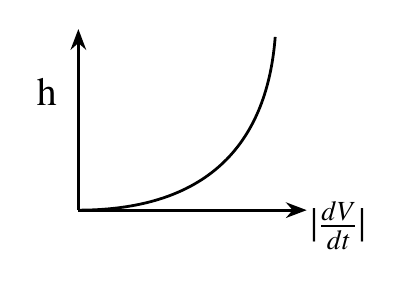
\begin{tikzpicture}[scale = 0.4]
		\tikzstyle{every node}=[font=\Large]
		\draw [line width=1pt, ->, >=Stealth] (7.5,11.5) -- (7.5,17.25);
		\draw [line width=1pt, ->, >=Stealth] (7.5,11.5) -- (14.75,11.5);
		\node [font=\Large] at (6.5,15.25) {h};
		\node [font=\Large] at (15.75,11) {$|\frac{dV}{dt}|$};
		\draw [line width=1pt, short] (7.5,11.5) .. controls (11.75,11.5) and (13.5,13.75) .. (13.75,17);
		\end{tikzpicture}
	
	\item 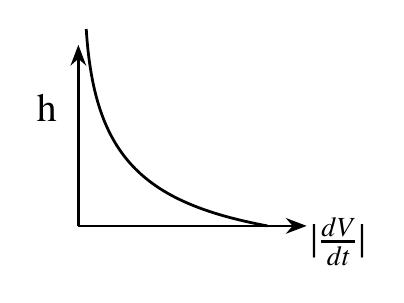
\begin{tikzpicture}[scale = 0.4]
		\tikzstyle{every node}=[font=\Large]
		\draw [line width=1pt, ->, >=Stealth] (7.5,11.5) -- (7.5,17.25);
		\draw [line width=1pt, ->, >=Stealth] (7.5,11.5) -- (14.75,11.5);
		\node [font=\Large] at (6.5,15.25) {h};
		\node [font=\Large] at (15.75,11) {$|\frac{dV}{dt}|$};
		\draw [line width=1pt, short] (7.75,17.75) .. controls (8,13.75) and (9.5,12.25) .. (13.5,11.5);
		\end{tikzpicture}

	
	\item 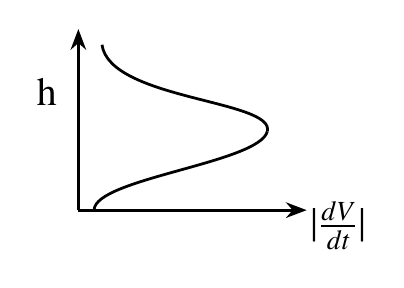
\begin{tikzpicture}[scale = 0.4]
		\tikzstyle{every node}=[font=\Large]
		\draw [line width=1pt, ->, >=Stealth] (7.5,11.5) -- (7.5,17.25);
		\draw [line width=1pt, ->, >=Stealth] (7.5,11.5) -- (14.75,11.5);
		\node [font=\Large] at (6.5,15.25) {h};
		\node [font=\Large] at (15.75,11) {$|\frac{dV}{dt}|$};
		\draw [line width=1pt, short] (8.25,16.75) .. controls (8.5,15) and (13.75,15) .. (13.5,14);
		\draw [line width=1pt, short] (13.5,14) .. controls (13.25,13) and (8,12.5) .. (8,11.5);
		\end{tikzpicture}

\end{enumerate}

\item Which of the following statement(s) is/are true about harmonically excited forced vibration of a single degree-of-freedom linear spring-mass-damper system?

\begin{enumerate}
	\item The total response of the mass is a combination of free vibration transient and steady-state response.
	\item The free vibration transient dies out with time for each of the three possible conditions of damping (under-damped, critically damped, and over-damped).
	\item The steady-state periodic response is dependent on the initial conditions at the time of application of external forcing.
	\item The rate of decay of free vibration transient response depends on the mass, spring stiffness and damping constant.
\end{enumerate}

\item Which of the following statement(s) is/are true about the state of stress in a plane?

\begin{enumerate}
	\item Maximum or major principal stress is algebraically the largest direct stress at a point.
	\item The magnitude of minor principal stress cannot be greater than the magnitude of major principal stress.
	\item The planes of maximum shear stress are inclined at 90 degrees to the principal axes.
	\item The normal stresses along the planes of maximum shear stress are equal.
\end{enumerate}

\end{enumerate}
\end{document}


